\chapter{Scenary}

	\section{Introduction}
		Each Scenary is built using a \emph{Tileset}. A Scenary have a number $Y$ of vertical cells and a number $X$ of horizontal cells. Each cell is a reference (pointer) to an \emph{Tile} of the Scenary \emph{Tileset}.
	\section{The Scenary}
		A Scenary is a matrix of Tiles (see \ref{tileset}) called cells. The cells starts from 0 -- height, and 0 -- width. The first cell is upper left corner, as shows fig \ref{fig:scenary}. Each \emph{Scenary} has a tileset, a \emph{Background} and  a visualisation window of $x$ by $y$ pixels wich moves across the scenary and try to center the character. 
		
		\begin{figure}[H]
			\centering
			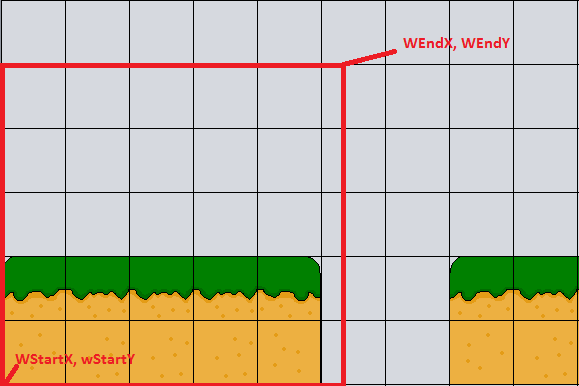
\includegraphics[width=\textwidth]{img/scenary.png}
			\caption{The scenary have a ``moving window'' next to character.}
			\label{fig:scenary}
		\end{figure}
		
		In  game, all scenaries have the same tile size and the same window size. The window is computed using the internal size. If an scenary have $10 \times 200$ tiles and each tile have $32$ pixels, the scenary size will be $320 \times 6400$ pixels, thus, the window size should consider this dimensions. Each window will be resized to fit the \emph{screen resolution} as show Figure \ref{fig:display}.
		
		\begin{figure}[H]
			\centering
			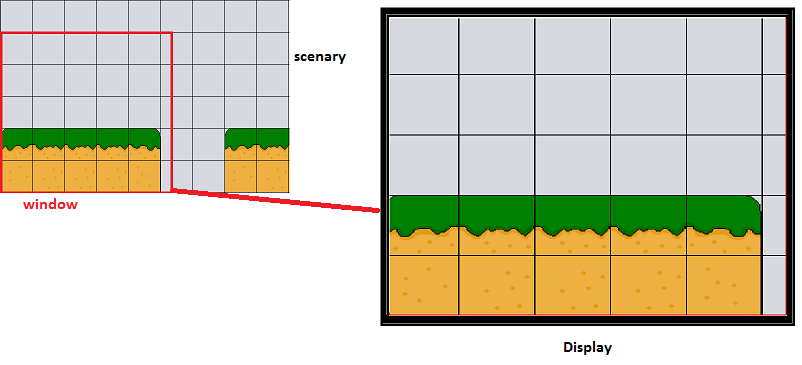
\includegraphics[width=\textwidth]{img/display.png}
			\caption{The buffer is resized to fill up the screen.}
			\label{fig:display}
		\end{figure}
	
		And the scenary coordinate system starts with (X,Y) -- at left bottom, and ends with (X,Y) -- at right upper, as shows Figure \ref{}.
		
		\begin{figure}[H]
			\centering
			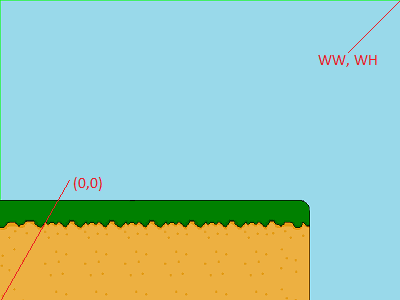
\includegraphics[]{img/scenarycoordinates.png}
			\caption{}
			\label{fig:scenarycoordinates}
		\end{figure}
		
	\section{File Format}
	
	\begin{algorithm}[H]
	\caption{Scenary File Format.}
	  \label{listing-scenaryFormat}
	  \begin{algorithmic}
		\STATE $SAVE\_TILESET()$
		\STATE $SAVE\_BACKGROUND()$
		\STATE $[int]internal\_window\_height$
		\STATE $[int]internal\_window\_width$
		\STATE $[double]gravity$
		\STATE $[int]tile\_number\_y$
		\STATE $[int]tile\_number\_x$
		
		
		\FOR{$i=0 \dots Number\_tiles\_Y$}
			\FOR{$i=0 \dots Number\_tiles\_X$}
				\STATE $a \gets 2$
			\ENDFOR
		\ENDFOR
	  \end{algorithmic}
	 \end{algorithm}